\documentclass[english]{../thermomemo/thermomemo}
% NOTE: You must pass either norsk or english as an option!
\usepackage[utf8]{inputenc}

\title{Testing the Lee-Kesler equation of state implementation in ThermoPack}
\author{Morten Hammer}

\usepackage[normalem]{ulem}
\usepackage{hyperref}
\usepackage{color}
\usepackage{amsmath}
\usepackage{graphicx}
%\usepackage[norsk]{babel}
\usepackage{setspace}
\usepackage{float}
%\newcommand{\HRule}{\rule{\linewidth}{0.5mm}}
\numberwithin{equation}{section}
\usepackage{mathtools}
\usepackage{rotating}
\usepackage{verbatim}
\usepackage{subcaption,caption}
\usepackage{todonotes}
\usepackage{xspace}

\newcommand*{\pd}[2]{\frac{\partial #1}{\partial #2}}
\newcommand*{\pdd}[2]{\frac{\partial^2 #1}{\partial #2^2}}
\newcommand*{\pder}[2]{\left(\frac{\partial #1}{\partial #2}\right)}
\newcommand*{\pdder}[2]{\left(\frac{\partial^2 #1}{\partial
      #2^2}\right)}
\newcommand*{\pddder}[2]{\left(\frac{\partial^3 #1}{\partial #2^3}\right)}
\newcommand*{\pdcross}[3]{\left(\frac{\partial^2 #1}{\partial #2 \partial #3}\right)}
\newcommand*{\reff}[1]{(\ref{#1})}

\newcommand*{\coto}{\ensuremath{\text{CO}_{\text{\scriptsize
        2}}}\xspace}
\newcommand*{\nto}{\ensuremath{\text{N}_{\text{\scriptsize
        2}}}\xspace}

\definecolor{midnightblue}{RGB}{35,35,132}
\definecolor{urlblue}{RGB}{70,130,180}

\hypersetup{
    colorlinks=true,
    linkcolor=midnightblue,
    urlcolor=urlblue,
    citecolor=midnightblue,
    linktoc=page
}

\usepackage[activate={true,nocompatibility},final,kerning=true,tracking=true,spacing=true,stretch=10,shrink=10]{microtype}
\microtypecontext{spacing=nonfrench}
\SetExtraKerning[unit=space]
    {encoding={*}, family={bch}, series={*}, size={footnotesize,small,normalsize}}
    {\textendash={400,400}, % en-dash, add more space around it
     "28={ ,150}, % left bracket, add space from right
     "29={150, }, % right bracket, add space from left
     \textquotedblleft={ ,150}, % left quotation mark, space from right
     \textquotedblright={150, }} % right quotation mark, space from left
\SetTracking{encoding={*}, shape=sc}{0}

\graphicspath{{gfx/}}

\begin{document}
\frontmatter

\tableofcontents

\section{Introduction}
Modifications of the work by J\o rgen R\o ysland Aarnes on the
Lee-Kesler equation of state (EoS) \cite{LK}. 

\section{The Lee-Kesler model}
The corresponding state method weigh the properties of two separate
equations of state as follows,
\begin{equation}
\label{eq:LK_main}
M = M^{(0)} + \frac{\omega_M}{\omega^{(r)}}(M^{(r)} - M^{(0)}),
\end{equation}
where, $\omega_M=\omega_M(\textbf{n})$. $M$ is $z$, $A^R$, $S^R$,
$H^R$ or any property that can be derived from these without using
mole number differentials.

The binary interaction parameters of Plöcker et al. \cite{PKP} is
implemented, and used for the testing of the Lee-Kelser EoS.

\subsection{Residual Gibbs energy}
The residual Gibbs energy, $G^R$, or the mixture fugacity coefficient,
$\ln \Phi_M$, for the reference and simple fluid was not included in
the memo by J{\o}rgen.
\begin{align}
\label{def:G^R(T,P,n)}
\ln \Phi_M = \frac{G^R(T,P,\textbf{n})}{RT} &= \frac{A^R(T,V,\textbf{n})}{RT} + n\left(z - 1 -
  \ln(z)\right)\\
\pder{\ln \Phi_M}{T}_{P,\textbf{n}} &= -\frac{H^R}{RT^2}\\
\pder{\ln \Phi_M}{P}_{T,\textbf{n}} &= \frac{V^R}{RT} = \frac{V -
  V^{ig}}{RT} = n\frac{\left(z-1\right)}{P}\\
  \ln \phi_i = \pder{\ln \Phi_M}{n_i}_{T,P} & = \frac{1}{RT} \pder{A^R}{n_i}_{T,V} - \ln z\\
\end{align}

\subsection{The fugacities and differentials}
Knowing the residual Gibbs energy, for the simple and reference fluid,
the combined fugacities can be derived. The mixture fugacity become
\begin{equation}
\label{eq:LK_fugacity}
\ln \Phi_M = \ln \Phi_M^{(0)} + \frac{\omega_M}{\omega^{(r)}}\left(\ln \Phi_M^{(r)} - \ln \Phi_M^{(0)}\right).
\end{equation}
The component fugacities become
\begin{equation}
\label{eq:LK_comp_fugacity}
\ln \phi_i = \ln \phi_i^{(0)} + \frac{\omega_M}{\omega^{(r)}}\left(\ln
\phi_i^{(r)} - \ln \phi_i^{(0)}\right) + \frac{1}{\omega^{(r)}}\pder{\omega_M}{n_i}\left(\ln \Phi_M^{(r)} - \ln \Phi_M^{(0)}\right).
\end{equation}
Further the differentials become
\begin{align}
\label{eq:LK_comp_fugacity_diff}
\pder{\ln \phi_i}{T}_{P} =& \pder{\ln \phi_i}{T}_{P}^{(0)} +
\frac{\omega_M}{\omega^{(r)}}\left(\pder{\ln \phi_i}{T}_{P}^{(r)} -
\pder{\ln \phi_i}{T}_{P}^{(0)}\right) \\
&+ \frac{1}{\omega^{(r)}}\pder{\omega_M}{n_i}\left(\pder{\ln
  \Phi_M}{T}_{P}^{(r)} - \pder{\ln \Phi_M}{T}_{P}^{(0)}\right), \\
\pder{\ln \phi_i}{P}_{T} =& \pder{\ln \phi_i}{P}_{T}^{(0)} +
\frac{\omega_M}{\omega^{(r)}}\left(\pder{\ln \phi_i}{P}_{T}^{(r)} -
\pder{\ln \phi_i}{P}_{T}^{(0)}\right) \\ 
&+ \frac{1}{\omega^{(r)}}\pder{\omega_M}{n_i}\left(\pder{\ln
  \Phi_M}{P}_{T}^{(r)} - \pder{\ln \Phi_M}{P}_{T}^{(0)}\right), \\
\ln \phi_{ij} =& \ln \phi_{ij}^{(0)} +
\frac{\omega_M}{\omega^{(r)}}\left(\ln \phi_{ij}^{(r)} - \ln
\phi_{ij}^{(0)}\right) + \frac{1}{\omega^{(r)}}\pder{\omega_M}{n_i}\left(\ln
\phi_j^{(r)} - \ln \phi_j^{(0)}\right)\\ 
& + \frac{1}{\omega^{(r)}}\pdcross{\omega_M}{n_i}{n_j}\left(\ln \Phi_M^{(r)} - \ln
\Phi_M^{(0)}\right). \\
\end{align}

\subsection{The residual entropy, enthalpy and differentials}
The combined residual entropy and enthalpy differentials will have the
same terms, so only the entropy and differentials are given. The
combined entropy is given as follows,
\begin{equation}
\label{eq:LK_entropy}
S^R(T,P,\textbf{n}) = S^R(T,P,\textbf{n})^{(0)} + \frac{\omega_M}{\omega^{(r)}}\left(S^R(T,P,\textbf{n})^{(r)} - S^R(T,P,\textbf{n})^{(0)}\right).
\end{equation}

To avoid too many superscripts, the residual, $R$, superscript is
dropped for the differentials of the entropy:
\begin{align}
\label{eq:LK_entropy_diff}
\pder{S}{T}_{P} &= \pder{S}{T}_{P}^{(0)} +
\frac{\omega_M}{\omega^{(r)}}\left(\pder{S}{T}_{P}^{(r)} -
\pder{S}{T}_{P}^{(0)}\right), \\
\pder{S}{P}_{T} &= \pder{S}{P}_{T}^{(0)} +
\frac{\omega_M}{\omega^{(r)}}\left(\pder{S}{P}_{T}^{(r)} -
\pder{S}{P}_{T}^{(0)}\right), \\
\pder{S}{n_i}_{T,P} &= \pder{S}{n_i}_{T,P}^{(0)} +
\frac{\omega_M}{\omega^{(r)}}\left(\pder{S}{n_i}_{T,P}^{(r)} -
\pder{S}{n_i}_{T,P}^{(0)}\right) +
\frac{1}{\omega^{(r)}}\pder{\omega_M}{n_i}\left(S^{(r)} - S^{(0)}\right)\\
\end{align}

\section{Modifications to the Lee-Kesler reduced specific volume solver}
Instead of solving directly for the reduced volume, $v_r(T_r,P_r)$, a solver
for the compressibility factor, $z$, is used. In order to determine the
compressibility factor, given $T_r$ and $P_r$ the following equation
must be solved,
\begin{equation}
\label{eq:LK_z_fun}
f(z) = z - \left[1 - \frac{v_r}{n} \left( \frac{\partial F}{\partial v_r} \right)_{T_r, \textbf{n}} \right] = 0,
\end{equation}
where $z=v_rP_r/T_r$.

To get good performance a third order method should be used. A third
order method require $f(z)$, $\partial f/ \partial z$, $\partial^2
f / \partial z^2$:
\begin{align}
\label{eq:LK_z_fun_diff}
\pder{f}{z} &= 1 + \frac{T_r}{P_r n} \left[\pder{F}{v_r}_{T_r, \textbf{n}} + v_r\pdder{F}{v_r}_{T_r, \textbf{n}}\right],\\
\pdder{f}{z} &= \frac{T_r^2}{P_r^2 n} \left[2\pdder{F}{v_r}_{T_r,
    \textbf{n}} + v_r \pddder{F}{v_r}_{T_r, \textbf{n}}\right].\\
\end{align}
In order to calculate these differentials, the third differential of
$F$ with respect to reduced specific volume, $\partial^3
F/ \partial v_r^3$, is required:
\begin{align}
\label{eq:LK_FDiff3vr}
\pddder{F}{v_r}_{T_r, \textbf{n}} =& n \bigg[-\frac{6B}{v_r^4} - \frac{12C}{v_r^5} - \frac{42D}{v_r^8} \\
  & - \frac{E}{v_r^5} \left(12\beta + \frac{(30 - 18\beta)\gamma}{v_r^2} + \frac{\left(4\beta-26\right)\gamma^2}{v_r^4} + \frac{4\gamma^3}{v_r^6} \right) \exp \left(-\frac{\gamma}{v_r^2} \right)\bigg]. \\
\end{align}

A Taylor expansion of $f$ is used to calculate the next step, $\Delta
z = z_{n+1} - z_n $, of the numerical procedure,
\begin{equation}
\label{eq:LK_z_fun_taylor}
f(z) = f(z_n) + f'(z_n)\Delta z + \frac{1}{2}f''(z_n)\Delta z = 0.
\end{equation}
The root giving the smallest change in z is selected, and the
series approximation,
\begin{equation}
\label{eq:LK_sqrt_series}
1 - \sqrt{1 - \alpha} = \frac{\alpha}{2} + \frac{\alpha^2}{8} + O(\alpha^3),
\end{equation}
is used to simplify the expression, and to avoid taking the square
root. We end up with the following step,
\begin{equation}
\label{eq:LK_z_step}
\Delta z = z_{n+1} - z_{n} = - \frac{f(z_{n})}{f'(z_{n})}\left(1+\frac{f(z_{n})f''(z_{n})}{f'(z_{n})^2}\right).
\end{equation}

\subsection{Selecting the correct roots of the simple and reference fluid}
In order to get physical values for the fugacities, the roots from
$f(z)$ for the simple and reference fluid must be selected
carefully. The simple fluid and reference fluid either have 1 or two
physical roots. If both the simple and reference fluid have a liquid
root, this is used. If both the simple and reference fluid have a gas
root, this is used. If the simple fluid have two roots, but the
reference fluid only have a liquid root, then the liquid root is
selected from both fluids, etc. 

In some situations, the simple fluid only have a gas root, and the
reference fluid only have a liquid root, see Figure \ref{fig:roots}. In
this situation, these roots are combined. 
\begin{figure}[h]
  \begin{subfigure}[b]{0.45\linewidth}
    \centering
    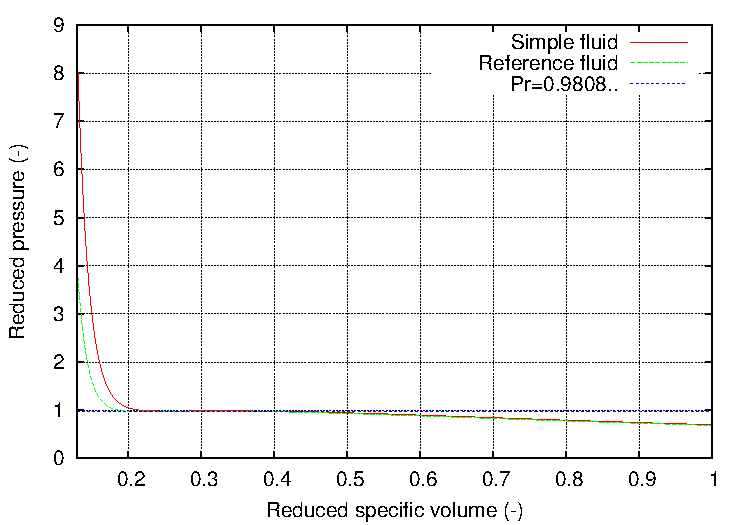
\includegraphics[width=1.0\textwidth]{roots}
    \caption{Reduced pressure vs. reduced specific volume}
    \label{fig:roots_a}
  \end{subfigure}
  \hfill
  \begin{subfigure}[b]{0.45\linewidth}
    \centering
    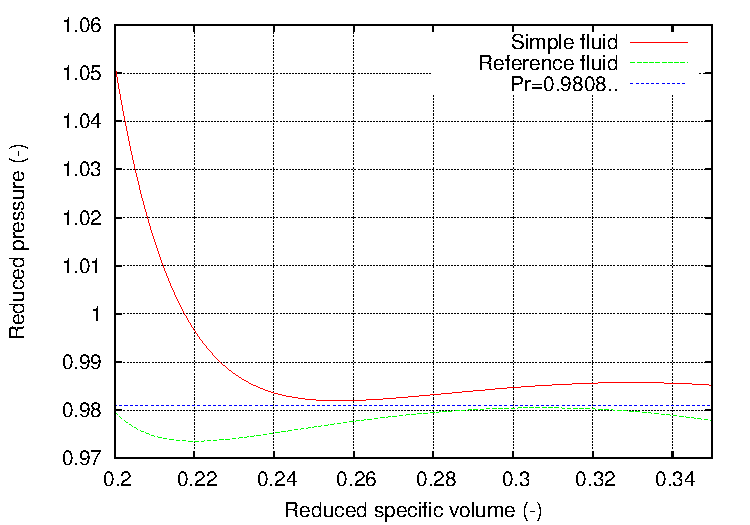
\includegraphics[width=1.0\textwidth]{roots_zoom}
    \caption{Reduced pressure vs. reduced specific volume. Zoomed
      version of Figure \ref{fig:roots_a}}
    \label{fig:roots_b}
  \end{subfigure}
  \caption{Reduced pressure $P_r$ as a function of reduced specific
    volume, for $T_r = 0.9973..$. For $P_r = 0.9808..$ it is seen that the
    simple fluid has a gas root, while the reference fluid has a liquid root.}
  \label{fig:roots}
\end{figure}

\section{Testing}
The entropies and enthalpies are tested for consistency, by comparing
$G^R$ with $H^R-TS^R$. The ideal contribution is calculated using the
$Cp$ polinomials already implemented in ThermoPack. 
\subsection{TP-flash using the Lee-Kesler EoS}
To test the Lee-Kesler implementation, a mixture of \coto and \nto is
used. The phase diagram, as calculated by the TP-flash, is shown in
Figure \ref{fig:co2n2}.
\begin{figure}[h]
  \centering
  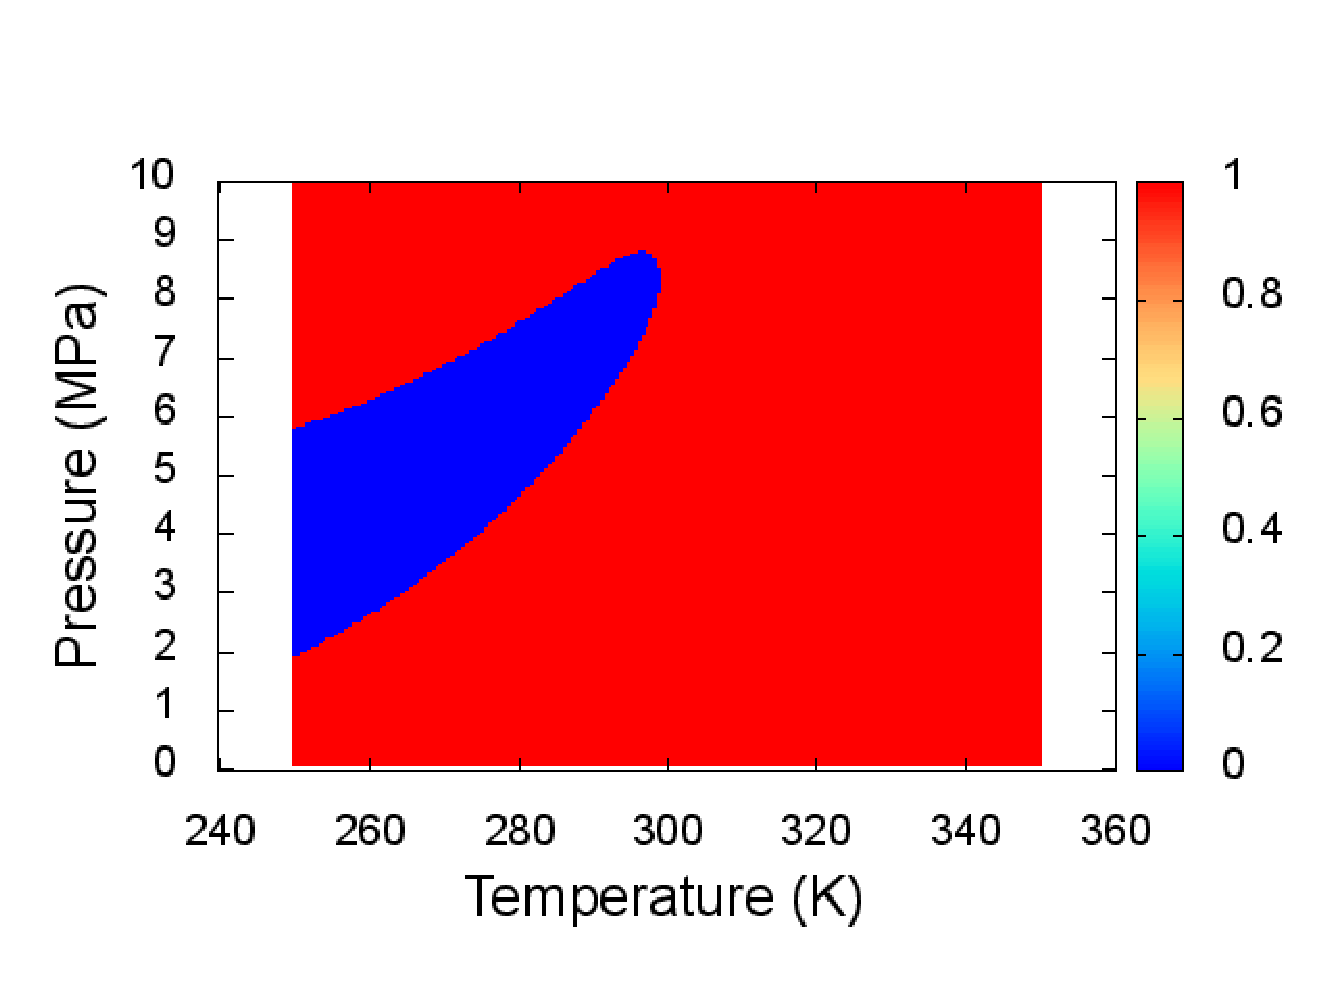
\includegraphics[width=0.8\textwidth]{co2n2}
  \caption{Phase diagram of \coto-\nto mixture, as calculated by the TP-flash,
  with 95 mass \% \coto. The blue area is the two-phase gas-liquid area.}
  \label{fig:co2n2}
\end{figure}

\section{Further work}
The Lee-Kesler implementation need more testing, and it is also
interesting to see how the models performes for densities of high
pressure \coto-mixtures. Some further work is listed below.
\begin{itemize}
\item Further testing to ensure robustness of the TP-flash
\item Test HP, SP and UV flash using Lee-Kesler EoS
\item Add a function to solve the EoS, returning the minimum Gibbs
  single phase solution. Test how close the solutions, $z_1$ and
  $z_2$, are. Use,
  \begin{equation}
    \frac{|z_1-z_2|}{\text{max}(z_1,z_2)} < \epsilon,
  \end{equation}
  where $\epsilon$ is the tolerance for the compressibillity solver.
\end{itemize}

\begin{thebibliography}{9}
  
\bibitem{LK}
	Lee, B.I., Kesler, M.G., \textit{A Generalized thermodynamic correlation based on a three-parameter corresponding states}, AlChE Journal, 21 (3), 510 (1975)

\bibitem{PKP}
	Plöcker, U., Knapp, H., Prausnitz, J., \textit{Calculations of High-Pressure Vapor-Liquid Equilibria from a Corresponding-States Correlation with Emphasis on Asymmetric Mixtures}, Ind. Eng. Chem. Process Des. Dev, 17 (3) 324 (1978)
	

\end{thebibliography}
\end{document}
